\documentclass{beamer}

\usepackage{graphicx,hyperref,udesc,url}
\usepackage[utf8]{inputenc}
\usepackage[T1]{fontenc}
\usepackage{booktabs}
\usepackage[portuges]{babel}


\title[Project Euler]{Aventuras no Project Euler:}
\subtitle{Ou como eu ganhei uma tatuagem de graça}

\author[Renan S. Silva]{{\small \url{uber.renan@gmail.com}}}

\institute[UDESC]{Departamento de Ci\^encia da Computa\c{c}\~ao \\
    Centro de Ci\^encias e Tecnol\'ogias\\
Universidade do Estado de Santa Catarina}

\begin{document}

\begin{frame}
    \titlepage

\end{frame}

\section{Introdução}
\begin{frame}
    \frametitle{Quem Sou}

    \begin{itemize}
        \item Cursando o 7º semestre(4-8 Fase) do BCC
        \item Speedcuber
        \item Origamista
        \item IC na área de Otimização Combinatorial
    \end{itemize}
\end{frame}

\begin{frame}
    \frametitle{Project Euler}
    O que é?

    \begin{itemize}
        \item Começou com Colin Hughes (a.k.a euler) no \url{http://mathschallenge.net/} (RIP)
        \item Tornou-se um projeto própio em 2006.
        \item É uma série de problemas envolvendo matemática e computação.
        \item Todos os problemas podem ser resolvidos em menos de 1 minuto.
        \item 1 problema novo toda semana.
    \end{itemize}
\end{frame}

\begin{frame}
    \frametitle{Project Euler}

    \begin{center}
        \textit{
            "Project Euler exists to encourage, challenge, and develop the skills and enjoyment of anyone with an interest in the fascinating world of mathematics."
        }
    \end{center}
\end{frame}

\begin{frame}
    \frametitle{Números}

    \begin{itemize}
        \item 600000 membros inscritos
        \item 7950000 Problemas resolvidos
        \item Média de 13.3 por membro
        \item 82000 membros resolveram pelo menos 25 problemas (13.7\%)
        \item 60 membros resolveram 500 problemas ou mais (561 problemas ao todo)
    \end{itemize}

    Linguagens mais usadas: Python, C/C++, Java, C\#, Haskell
\end{frame}

\begin{frame}
    \frametitle{Mais números}

    \begin{figure}[htpb]
        \centering
        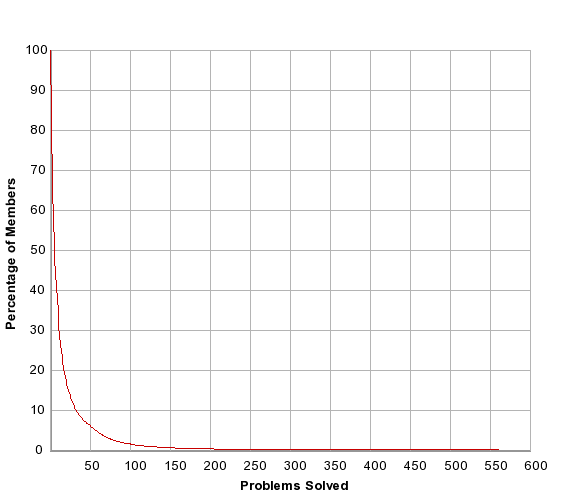
\includegraphics[width=0.8\linewidth]{images/graph1.png}
        \caption{images/Graph1}
        \label{fig:images/graph1}
    \end{figure}
\end{frame}

\begin{frame}
    \frametitle{Mais números}

    \begin{figure}[htpb]
        \centering
        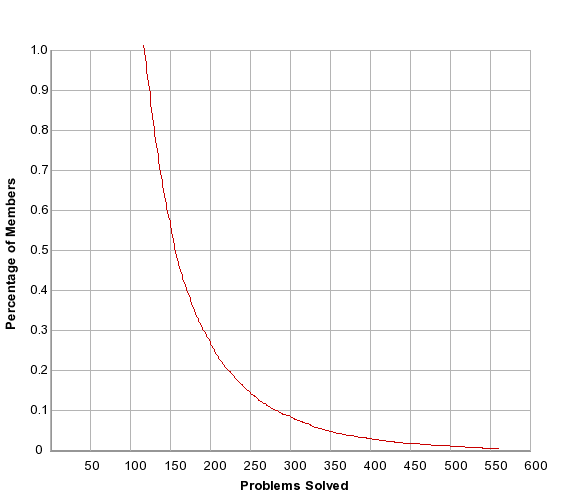
\includegraphics[width=0.8\linewidth]{images/graph2.png}
        \caption{images/Graph2}
        \label{fig:images/graph2}
    \end{figure}
\end{frame}

\begin{frame}
    \frametitle{Top 100}

    Top 100 de alguns países:

\begin{table}[htpb]
    \centering
    \begin{tabular}{c c c}
        País             & Mínimo para o top 100 & Membros ativos \\
        USA              & 256                   & 37527 \\
        Holanda          & 106                   & 3508 \\
        França           & 148                   & 4419 \\
        Russia           & 119                   & 4419 \\
        Brazil           & 35                    & 3110 \\
        República Tcheca & 37                    & 1087 \\
    \end{tabular}
\end{table}

\end{frame}

\begin{frame}
    \frametitle{Ranking Brasileiro}
\begin{figure}[htpb]
    \centering
    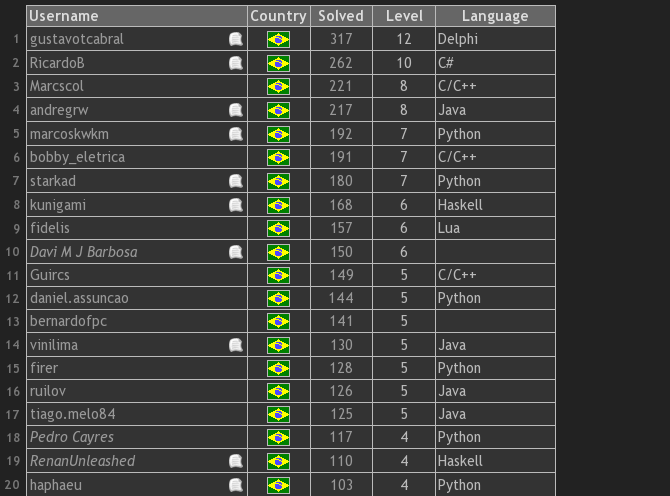
\includegraphics[width=0.8\linewidth]{images/top20_br.png}
\end{figure}
\end{frame}

\begin{frame}
    \frametitle{Titulo}

\end{frame}


\begin{frame}
    \frametitle{Titulo}

\end{frame}

\section{Isso é outra seção}
\begin{frame}
    \frametitle{Isso é um titulo}

    Isso é um texto.
    \begin{itemize}
        \item Isso é um item;
        \item PogChamp;
        \item Kappa;
        \item KTHXBYE;
    \end{itemize}
\end{frame}

\end{document}
